\chapter{Gal}
\section{Zähler}
\subsection{Mealy-Automat}
Als Hilfe zum Aufstellen einer Wahrheitswerttabelle für den internen Zähler, haben wir erst einen
Mealy-Automaten entworfen.

\begin{figure}[H]
    \centering
    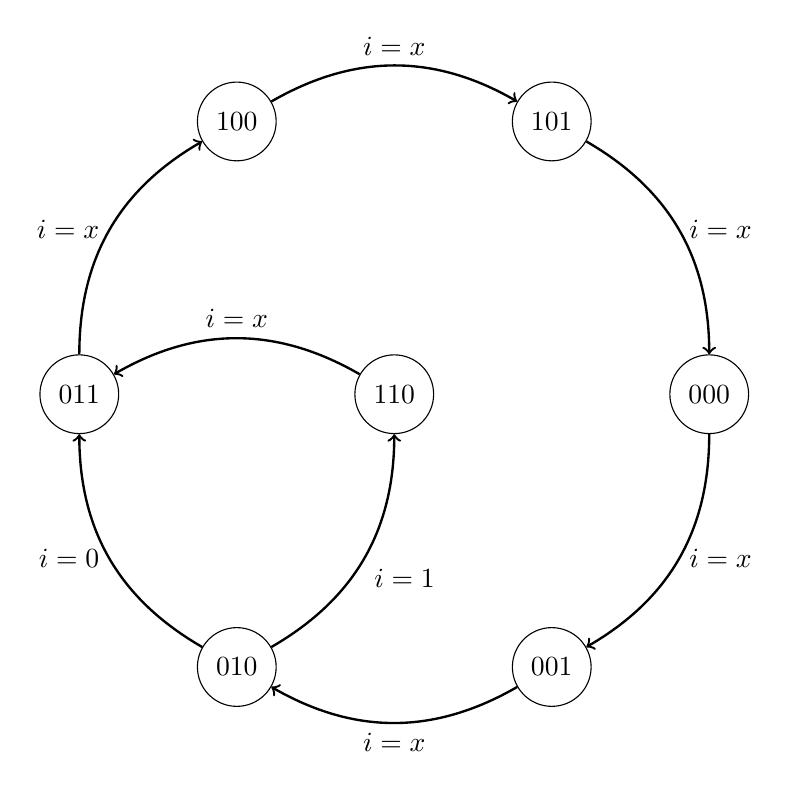
\begin{tikzpicture}
        \node[circle, draw, minimum size=1cm] (N0) at (0:4cm) {$000$};
        \node[circle, draw, minimum size=1cm] (N1) at (300:4cm) {$001$};
        \node[circle, draw, minimum size=1cm] (N2) at (240:4cm) {$010$};
        \node[circle, draw, minimum size=1cm] (N3) at (180:4cm) {$011$};
        \node[circle, draw, minimum size=1cm] (N4) at (120:4cm) {$100$};
        \node[circle, draw, minimum size=1cm] (N5) at (60:4cm) {$101$};
        \node[circle, draw, minimum size=1cm] (N6) at (0,0) {$110$};

        \path[->,line width=0.3mm]
        (N0) edge[bend left] node[right] {$i=x$} (N1)
        (N1) edge[bend left] node[below] {$i=x$} (N2)
        (N2) edge[bend left] node[left] {$i=0$} (N3)
        (N2) edge[bend right] node[below right] {$i=1$} (N6)
        (N3) edge[bend left] node[left] {$i=x$} (N4)
        (N4) edge[bend left] node[above] {$i=x$} (N5)
        (N5) edge[bend left] node[right] {$i=x$} (N0)
        (N6) edge[bend right] node[above] {$i=x$} (N3);
    \end{tikzpicture}
    \label{fig:gal-stateMachine}
\end{figure}

\newpage

\subsection{Wahrheitswerttabelle}
Aus dem Automaten \ref{fig:gal-stateMachine} lässt sich leicht die Wahrheitswerttabelle für den Zähler 
ablesen. Diese finden Sie im Anschluss.

\begin{table}[H]
    \centering
    \def\arraystretch{1.3}
    \rowcolors{2}{gray!15}{white}
    \begin{tabular}{|c!{\vrule width 1.5pt}c|c|c|c!{\vrule width 1.5pt}c|c|c|}
        \rowcolor{gray!50}
        \hline
        Dez. & $z_2$ & $z_1$ & $z_0$ & $i$ & $z_2^+$ & $z_1^+$ & $z_0^+$ \\
        \hline
        0    & 0     & 0     & 0     & 0   & 0       & 0       & 1       \\
        1    & 0     & 0     & 0     & 1   & 0       & 0       & 1       \\
        2    & 0     & 0     & 1     & 0   & 0       & 1       & 0       \\
        3    & 0     & 0     & 1     & 1   & 0       & 1       & 0       \\
        4    & 0     & 1     & 0     & 0   & 0       & 1       & 1       \\
        5    & 0     & 1     & 0     & 1   & 1       & 1       & 0       \\
        6    & 0     & 1     & 1     & 0   & 1       & 0       & 0       \\
        7    & 0     & 1     & 1     & 1   & 1       & 0       & 0       \\
        8    & 1     & 0     & 0     & 0   & 1       & 0       & 1       \\
        9    & 1     & 0     & 0     & 1   & 1       & 0       & 1       \\
        10   & 1     & 0     & 1     & 0   & 0       & 0       & 0       \\
        11   & 1     & 0     & 1     & 1   & 0       & 0       & 0       \\
        12   & 1     & 1     & 0     & 0   & 0       & 1       & 1       \\
        13   & 1     & 1     & 0     & 1   & 0       & 1       & 1       \\
        14   & 1     & 1     & 1     & 0   & x       & x       & x       \\
        15   & 1     & 1     & 1     & 1   & x       & x       & x       \\
        \hline
    \end{tabular}
    \label{tab:gal-counter-truthtable}
\end{table}

\newpage

\subsection{KV-Diagramme und vereinfachte Formeln}
Hier entwickeln wir die vereinfachten Formeln, welche aus der Wahrheitswerttabelle \ref{tab:gal-counter-truthtable} folgen.

\begin{table}[H]
    \centering
    \renewcommand{\arraystretch}{7.5}
    \begin{tabular}{c@{\hskip 1.5cm}c}
        \begin{tikzpicture}
            \matrix[matrix of nodes, nodes={draw, minimum size=1cm, anchor=center, text height=1.5ex, text depth=.25ex}] (kmap) {
            |[]| 0 & |[]| 0 & |[]| 0 & |[]| 0 \\
            |[]| 0 & |[]| 1 & |[]| 1 & |[]| 1 \\
            |[]| 0 & |[]| 0 & |[]| x & |[]| x \\
            |[]| 1 & |[]| 1 & |[]| 0 & |[]| 0 \\
            };

            % Add decimal numbers in the bottom right corner of each cell
            \foreach \i/\j/\num in {1/1/0, 1/2/1, 1/3/3, 1/4/2, 2/1/4, 2/2/5, 2/3/7, 2/4/6, 3/1/12, 3/2/13, 3/3/15, 3/4/14, 4/1/8, 4/2/9, 4/3/11, 4/4/10} {
                    \node[anchor=south east, font=\tiny] at (kmap-\i-\j.south east) {\num};
                }

            % Add variable names for rows
            \node[left=0.2cm of kmap-1-1.west] {$\overline{z}_2$};
            \node[left=0.2cm of kmap-2-1.west] {$\overline{z}_2$};
            \node[left=0.2cm of kmap-3-1.west] {$z_2$};
            \node[left=0.2cm of kmap-4-1.west] {$z_2$};

            % Add variable names for columns
            \node[above=0.2cm of kmap-1-1.north] {$\overline{i}$};
            \node[above=0.2cm of kmap-1-2.north] {$i$};
            \node[above=0.2cm of kmap-1-3.north] {$i$};
            \node[above=0.2cm of kmap-1-4.north] {$\overline{i}$};

            % Add variable names for rows on the right
            \node[right=0.2cm of kmap-1-4.east] {$\overline{z}_1$};
            \node[right=0.2cm of kmap-2-4.east] {$z_1$};
            \node[right=0.2cm of kmap-3-4.east] {$z_1$};
            \node[right=0.2cm of kmap-4-4.east] {$\overline{z}_1$};

            % Add variable names for columns on the bottom
            \node[below=0.2cm of kmap-4-1.south] {$\overline{z}_0$};
            \node[below=0.2cm of kmap-4-2.south] {$\overline{z}_0$};
            \node[below=0.2cm of kmap-4-3.south] {$z_0$};
            \node[below=0.2cm of kmap-4-4.south] {$z_0$};

            % Mark areas to simplify with multiple semi-transparent backgrounds
            \draw[fill=yellow, fill opacity=0.3, draw=none] (kmap-2-2.north west) rectangle (kmap-2-3.south east);
            \draw[fill=blue, fill opacity=0.3, draw=none] (kmap-2-3.north west) rectangle (kmap-3-4.south east);
            \draw[fill=green, fill opacity=0.2, draw=none] (kmap-4-1.north west) rectangle (kmap-4-2.south east);

            % Formula below
            \node[below=1cm of kmap] {$z_2^+ = \overline{z}_2 z_1 i \ \lor \ z_2 \overline{z}_1 \overline{z}_0 \ \lor \ z_1 z_0$};

        \end{tikzpicture} &
        \begin{tikzpicture}
            \matrix[matrix of nodes, nodes={draw, minimum size=1cm, anchor=center, text height=1.5ex, text depth=.25ex}] (kmap) {
            |[]| 0 & |[]| 0 & |[]| 1 & |[]| 1 \\
            |[]| 1 & |[]| 1 & |[]| 0 & |[]| 0 \\
            |[]| 1 & |[]| 1 & |[]| x & |[]| x \\
            |[]| 0 & |[]| 0 & |[]| 0 & |[]| 0 \\
            };

            % Add decimal numbers in the bottom right corner of each cell
            \foreach \i/\j/\num in {1/1/0, 1/2/1, 1/3/3, 1/4/2, 2/1/4, 2/2/5, 2/3/7, 2/4/6, 3/1/12, 3/2/13, 3/3/15, 3/4/14, 4/1/8, 4/2/9, 4/3/11, 4/4/10} {
                    \node[anchor=south east, font=\tiny] at (kmap-\i-\j.south east) {\num};
                }

            % Add variable names for rows
            \node[left=0.2cm of kmap-1-1.west] {$\overline{z}_2$};
            \node[left=0.2cm of kmap-2-1.west] {$\overline{z}_2$};
            \node[left=0.2cm of kmap-3-1.west] {$z_2$};
            \node[left=0.2cm of kmap-4-1.west] {$z_2$};

            % Add variable names for columns
            \node[above=0.2cm of kmap-1-1.north] {$\overline{i}$};
            \node[above=0.2cm of kmap-1-2.north] {$i$};
            \node[above=0.2cm of kmap-1-3.north] {$i$};
            \node[above=0.2cm of kmap-1-4.north] {$\overline{i}$};

            % Add variable names for rows on the right
            \node[right=0.2cm of kmap-1-4.east] {$\overline{z}_1$};
            \node[right=0.2cm of kmap-2-4.east] {$z_1$};
            \node[right=0.2cm of kmap-3-4.east] {$z_1$};
            \node[right=0.2cm of kmap-4-4.east] {$\overline{z}_1$};

            % Add variable names for columns on the bottom
            \node[below=0.2cm of kmap-4-1.south] {$\overline{z}_0$};
            \node[below=0.2cm of kmap-4-2.south] {$\overline{z}_0$};
            \node[below=0.2cm of kmap-4-3.south] {$z_0$};
            \node[below=0.2cm of kmap-4-4.south] {$z_0$};

            % Mark areas to simplify with multiple semi-transparent backgrounds
            \draw[fill=yellow, fill opacity=0.3, draw=none] (kmap-1-3.north west) rectangle (kmap-1-4.south east);
            \draw[fill=blue, fill opacity=0.3, draw=none] (kmap-2-1.north west) rectangle (kmap-3-2.south east);

            % Formula below
            \node[below=1cm of kmap] {$z_1^+ = z_1 \overline{z}_0 \ \lor \ \overline{z}_2 \overline{z}_1 z_0$};

        \end{tikzpicture}
        \\
        \begin{tikzpicture}
            \matrix[matrix of nodes, nodes={draw, minimum size=1cm, anchor=center, text height=1.5ex, text depth=.25ex}] (kmap) {
            |[]| 1 & |[]| 1 & |[]| 0 & |[]| 0 \\
            |[]| 1 & |[]| 0 & |[]| 0 & |[]| 0 \\
            |[]| 1 & |[]| 1 & |[]| x & |[]| x \\
            |[]| 1 & |[]| 1 & |[]| 0 & |[]| 0 \\
            };

            % Add decimal numbers in the bottom right corner of each cell
            \foreach \i/\j/\num in {1/1/0, 1/2/1, 1/3/3, 1/4/2, 2/1/4, 2/2/5, 2/3/7, 2/4/6, 3/1/12, 3/2/13, 3/3/15, 3/4/14, 4/1/8, 4/2/9, 4/3/11, 4/4/10} {
                    \node[anchor=south east, font=\tiny] at (kmap-\i-\j.south east) {\num};
                }

            % Add variable names for rows
            \node[left=0.2cm of kmap-1-1.west] {$\overline{z}_2$};
            \node[left=0.2cm of kmap-2-1.west] {$\overline{z}_2$};
            \node[left=0.2cm of kmap-3-1.west] {$z_2$};
            \node[left=0.2cm of kmap-4-1.west] {$z_2$};

            % Add variable names for columns
            \node[above=0.2cm of kmap-1-1.north] {$\overline{i}$};
            \node[above=0.2cm of kmap-1-2.north] {$i$};
            \node[above=0.2cm of kmap-1-3.north] {$i$};
            \node[above=0.2cm of kmap-1-4.north] {$\overline{i}$};

            % Add variable names for rows on the right
            \node[right=0.2cm of kmap-1-4.east] {$\overline{z}_1$};
            \node[right=0.2cm of kmap-2-4.east] {$z_1$};
            \node[right=0.2cm of kmap-3-4.east] {$z_1$};
            \node[right=0.2cm of kmap-4-4.east] {$\overline{z}_1$};

            % Add variable names for columns on the bottom
            \node[below=0.2cm of kmap-4-1.south] {$\overline{z}_0$};
            \node[below=0.2cm of kmap-4-2.south] {$\overline{z}_0$};
            \node[below=0.2cm of kmap-4-3.south] {$z_0$};
            \node[below=0.2cm of kmap-4-4.south] {$z_0$};

            % Mark areas to simplify with multiple semi-transparent backgrounds
            \draw[fill=yellow, fill opacity=0.3, draw=none] (kmap-1-1.north west) rectangle (kmap-4-1.south east);
            \draw[fill=blue, fill opacity=0.3, draw=none] (kmap-3-1.north west) rectangle (kmap-3-4.south east);
            \draw[fill=green, fill opacity=0.2, draw=none] (kmap-1-1.north west) rectangle (kmap-1-2.south east);
            \draw[fill=green, fill opacity=0.2, draw=none] (kmap-4-1.north west) rectangle (kmap-4-2.south east);

            % Formula below
            \node[below=1cm of kmap] {$z_0^+ = \overline{z}_0 \overline{i} \ \lor \ \overline{z}_1 \overline{z}_0 \ \lor \ z_2 z_1$};

        \end{tikzpicture}
    \end{tabular}
    \label{fig:gal-counter-karnaugMaps}
\end{table}

\newpage

\section{Mapping Zähler auf Würfel}
\subsection{Wahrheitswerttabelle}
Es sind nun die Zählerzustände \ref{fig:gal-counter-karnaugMaps} auf die Pins des Würfels abzubilden. Dafür haben wir die folgende Wahrheitswerttabelle aufgestellt.

\begin{table}[H]
    \centering
    \def\arraystretch{1.3}
    \rowcolors{2}{gray!15}{white}
    \begin{tabular}{|c|c!{\vrule width 1.5pt}c|c|c!{\vrule width 1.5pt}c|c|c|c|}
        \rowcolor{gray!50}
        \hline
        Dez. & WZ. & $z_2$ & $z_1$ & $z_0$ & $w_3$ & $w_2$ & $w_1$ & $w_0$ \\
        \hline
        0    & 1   & 0     & 0     & 0     & 1     & 1     & 1     & 0     \\
        1    & 2   & 0     & 0     & 1     & 1     & 1     & 0     & 1     \\
        2    & 3   & 0     & 1     & 0     & 1     & 1     & 0     & 0     \\
        3    & 4   & 0     & 1     & 1     & 1     & 0     & 0     & 1     \\
        4    & 5   & 1     & 0     & 0     & 1     & 0     & 0     & 0     \\
        5    & 6   & 1     & 0     & 1     & 0     & 0     & 0     & 1     \\
        6    & 6   & 1     & 1     & 0     & 0     & 0     & 0     & 1     \\
        \hline
    \end{tabular}
    \label{tab:gal-mapping-truthtable}
\end{table}

 \newpage

\subsection{KV-Diagramme und vereinfachte Formeln}
Aus Tabelle \ref{tab:gal-mapping-truthtable} ergeben sich die folgenden Formeln.
\begin{table}[H]
    \centering
    \renewcommand{\arraystretch}{7.5}
    \begin{tabular}{c@{\hskip 1.5cm}c}
        \begin{tikzpicture}
            \matrix[matrix of nodes, nodes={draw, minimum size=1cm, anchor=center, text height=1.5ex, text depth=.25ex}] (kmap) {
            |[]| 1 & |[]| 1 & |[]| 1 & |[]| 1 \\
            |[]| 1 & |[]| 0 & |[]| x & |[]| 0 \\
            };

            % Add decimal numbers in the bottom right corner of each cell
            \foreach \i/\j/\num in {1/1/0, 1/2/1, 1/3/3, 1/4/2, 2/1/4, 2/2/5, 2/3/7, 2/4/6} {
                    \node[anchor=south east, font=\tiny] at (kmap-\i-\j.south east) {\num};
                }

            % Add variable names for columns
            \node[above=0.2cm of kmap-1-1.north] {$\overline{z}_0$};
            \node[above=0.2cm of kmap-1-2.north] {$z_0$};
            \node[above=0.2cm of kmap-1-3.north] {$z_0$};
            \node[above=0.2cm of kmap-1-4.north] {$\overline{z}_0$};

            % Add variable names for columns on the bottom
            \node[below=0.2cm of kmap-2-1.south] {$\overline{z}_1$};
            \node[below=0.2cm of kmap-2-2.south] {$\overline{z}_1$};
            \node[below=0.3cm of kmap-2-3.south] {$z_1$};
            \node[below=0.3cm of kmap-2-4.south] {$z_1$};

            % Add variable names for rows on the right
            \node[right=0.2cm of kmap-1-4.east] {$\overline{z}_2$};
            \node[right=0.2cm of kmap-2-4.east] {$z_2$};

            % Mark areas to simplify with multiple semi-transparent backgrounds
            \draw[fill=yellow, fill opacity=0.3, draw=none] (kmap-1-1.north west) rectangle (kmap-1-4.south east);
            \draw[fill=blue, fill opacity=0.3, draw=none] (kmap-1-1.north west) rectangle (kmap-2-1.south east);

            % Formula below
            \node[below=1cm of kmap] {$w_3 = \overline{z}_2 \ \lor \ \overline{z}_1 \overline{z}_0$};

        \end{tikzpicture} &
        \begin{tikzpicture}
            \matrix[matrix of nodes, nodes={draw, minimum size=1cm, anchor=center, text height=1.5ex, text depth=.25ex}] (kmap) {
            |[]| 1 & |[]| 1 & |[]| 0 & |[]| 1 \\
            |[]| 0 & |[]| 0 & |[]| x & |[]| 0 \\
            };

            % Add decimal numbers in the bottom right corner of each cell
            \foreach \i/\j/\num in {1/1/0, 1/2/1, 1/3/3, 1/4/2, 2/1/4, 2/2/5, 2/3/7, 2/4/6} {
                    \node[anchor=south east, font=\tiny] at (kmap-\i-\j.south east) {\num};
                }

            % Add variable names for columns
            \node[above=0.2cm of kmap-1-1.north] {$\overline{z}_0$};
            \node[above=0.2cm of kmap-1-2.north] {$z_0$};
            \node[above=0.2cm of kmap-1-3.north] {$z_0$};
            \node[above=0.2cm of kmap-1-4.north] {$\overline{z}_0$};

            % Add variable names for columns on the bottom
            \node[below=0.2cm of kmap-2-1.south] {$\overline{z}_1$};
            \node[below=0.2cm of kmap-2-2.south] {$\overline{z}_1$};
            \node[below=0.3cm of kmap-2-3.south] {$z_1$};
            \node[below=0.3cm of kmap-2-4.south] {$z_1$};

            % Add variable names for rows on the right
            \node[right=0.2cm of kmap-1-4.east] {$\overline{z}_2$};
            \node[right=0.2cm of kmap-2-4.east] {$z_2$};

            % Mark areas to simplify with multiple semi-transparent backgrounds
            \draw[fill=yellow, fill opacity=0.3, draw=none] (kmap-1-1.north west) rectangle (kmap-1-2.south east);
            \draw[fill=blue, fill opacity=0.3, draw=none] (kmap-1-4.north west) rectangle (kmap-1-4.south east);
            \draw[fill=blue, fill opacity=0.3, draw=none] (kmap-1-1.north west) rectangle (kmap-1-1.south east);

            % Formula below
            \node[below=1cm of kmap] {$w_2 = \overline{z}_2 \overline{z}_0 \ \lor \ \overline{z}_2 \overline{z}_1$};

        \end{tikzpicture}
        \\
        \begin{tikzpicture}
            \matrix[matrix of nodes, nodes={draw, minimum size=1cm, anchor=center, text height=1.5ex, text depth=.25ex}] (kmap) {
            |[]| 1 & |[]| 0 & |[]| 0 & |[]| 0 \\
            |[]| 0 & |[]| 0 & |[]| x & |[]| 0 \\
            };

            % Add decimal numbers in the bottom right corner of each cell
            \foreach \i/\j/\num in {1/1/0, 1/2/1, 1/3/3, 1/4/2, 2/1/4, 2/2/5, 2/3/7, 2/4/6} {
                    \node[anchor=south east, font=\tiny] at (kmap-\i-\j.south east) {\num};
                }

            % Add variable names for columns
            \node[above=0.2cm of kmap-1-1.north] {$\overline{z}_0$};
            \node[above=0.2cm of kmap-1-2.north] {$z_0$};
            \node[above=0.2cm of kmap-1-3.north] {$z_0$};
            \node[above=0.2cm of kmap-1-4.north] {$\overline{z}_0$};

            % Add variable names for columns on the bottom
            \node[below=0.2cm of kmap-2-1.south] {$\overline{z}_1$};
            \node[below=0.2cm of kmap-2-2.south] {$\overline{z}_1$};
            \node[below=0.3cm of kmap-2-3.south] {$z_1$};
            \node[below=0.3cm of kmap-2-4.south] {$z_1$};

            % Add variable names for rows on the right
            \node[right=0.2cm of kmap-1-4.east] {$\overline{z}_2$};
            \node[right=0.2cm of kmap-2-4.east] {$z_2$};

            % Mark areas to simplify with multiple semi-transparent backgrounds
            \draw[fill=yellow, fill opacity=0.3, draw=none] (kmap-1-1.north west) rectangle (kmap-1-1.south east);

            % Formula below
            \node[below=1cm of kmap] {$w_1 = \overline{z}_2 \overline{z}_1 \overline{z}_0$};

        \end{tikzpicture} &
        \begin{tikzpicture}
            \matrix[matrix of nodes, nodes={draw, minimum size=1cm, anchor=center, text height=1.5ex, text depth=.25ex}] (kmap) {
            |[]| 0 & |[]| 1 & |[]| 1 & |[]| 0 \\
            |[]| 0 & |[]| 1 & |[]| x & |[]| 1 \\
            };

            % Add decimal numbers in the bottom right corner of each cell
            \foreach \i/\j/\num in {1/1/0, 1/2/1, 1/3/3, 1/4/2, 2/1/4, 2/2/5, 2/3/7, 2/4/6} {
                    \node[anchor=south east, font=\tiny] at (kmap-\i-\j.south east) {\num};
                }

            % Add variable names for columns
            \node[above=0.2cm of kmap-1-1.north] {$\overline{z}_0$};
            \node[above=0.2cm of kmap-1-2.north] {$z_0$};
            \node[above=0.2cm of kmap-1-3.north] {$z_0$};
            \node[above=0.2cm of kmap-1-4.north] {$\overline{z}_0$};

            % Add variable names for columns on the bottom
            \node[below=0.2cm of kmap-2-1.south] {$\overline{z}_1$};
            \node[below=0.2cm of kmap-2-2.south] {$\overline{z}_1$};
            \node[below=0.3cm of kmap-2-3.south] {$z_1$};
            \node[below=0.3cm of kmap-2-4.south] {$z_1$};

            % Add variable names for rows on the right
            \node[right=0.2cm of kmap-1-4.east] {$\overline{z}_2$};
            \node[right=0.2cm of kmap-2-4.east] {$z_2$};

            % Mark areas to simplify with multiple semi-transparent backgrounds
            \draw[fill=yellow, fill opacity=0.3, draw=none] (kmap-1-2.north west) rectangle (kmap-2-3.south east);
            \draw[fill=blue, fill opacity=0.3, draw=none] (kmap-2-3.north west) rectangle (kmap-2-4.south east);

            % Formula below
            \node[below=1cm of kmap] {$w_0 = z_0 \ \lor \ z_2 z_1$};

        \end{tikzpicture}
    \end{tabular}
    \label{gal-mapping-karnaugMaps}
\end{table}

\newpage

\section{Code}
Die Implementation der Formeln \ref{gal-mapping-karnaugMaps} im GAL können Sie dem folgenden Code-Block entnehmen.
\begin{tcolorbox}[colback=gray!10,colframe=black,boxrule=0.5pt]
\begin{verbatim}
PIN 1 = clock ;
PIN 2 = i ;

PIN 16 = z0 ; /* Pin nicht angeschlossen, fuer int. Funktion notwendig */
PIN 17 = z1 ; /* Pin nicht angeschlossen, fuer int. Funktion notwendig */
PIN 18 = z2 ; /* Pin nicht angeschlossen, fuer int. Funktion notwendig */

PIN 16 = w0 ;
PIN 17 = w1 ;
PIN 18 = w2 ;
PIN 19 = w3 ;

z2.d = !z2 & z1 & i # z2 & !z1 & !z0 # z1 & z0;
z1.d = z1 & !z0 # !z2 & !z1 & z0;
z0.d = !z0 & !i # !z1 & !z0 # z2 & z1;

w3.d = !z2 # !z1 & !z0;
w2.d = !z2 & !z0 # !z2 & !z1;
w1.d = !z2 & !z1 & !z0;
w0.d = z0 # z2 & z1;
\end{verbatim}
\end{tcolorbox}

\newpage

\section{Aufbau}
Der aufgebaute Gal.
\begin{figure}[H]
    \centering
     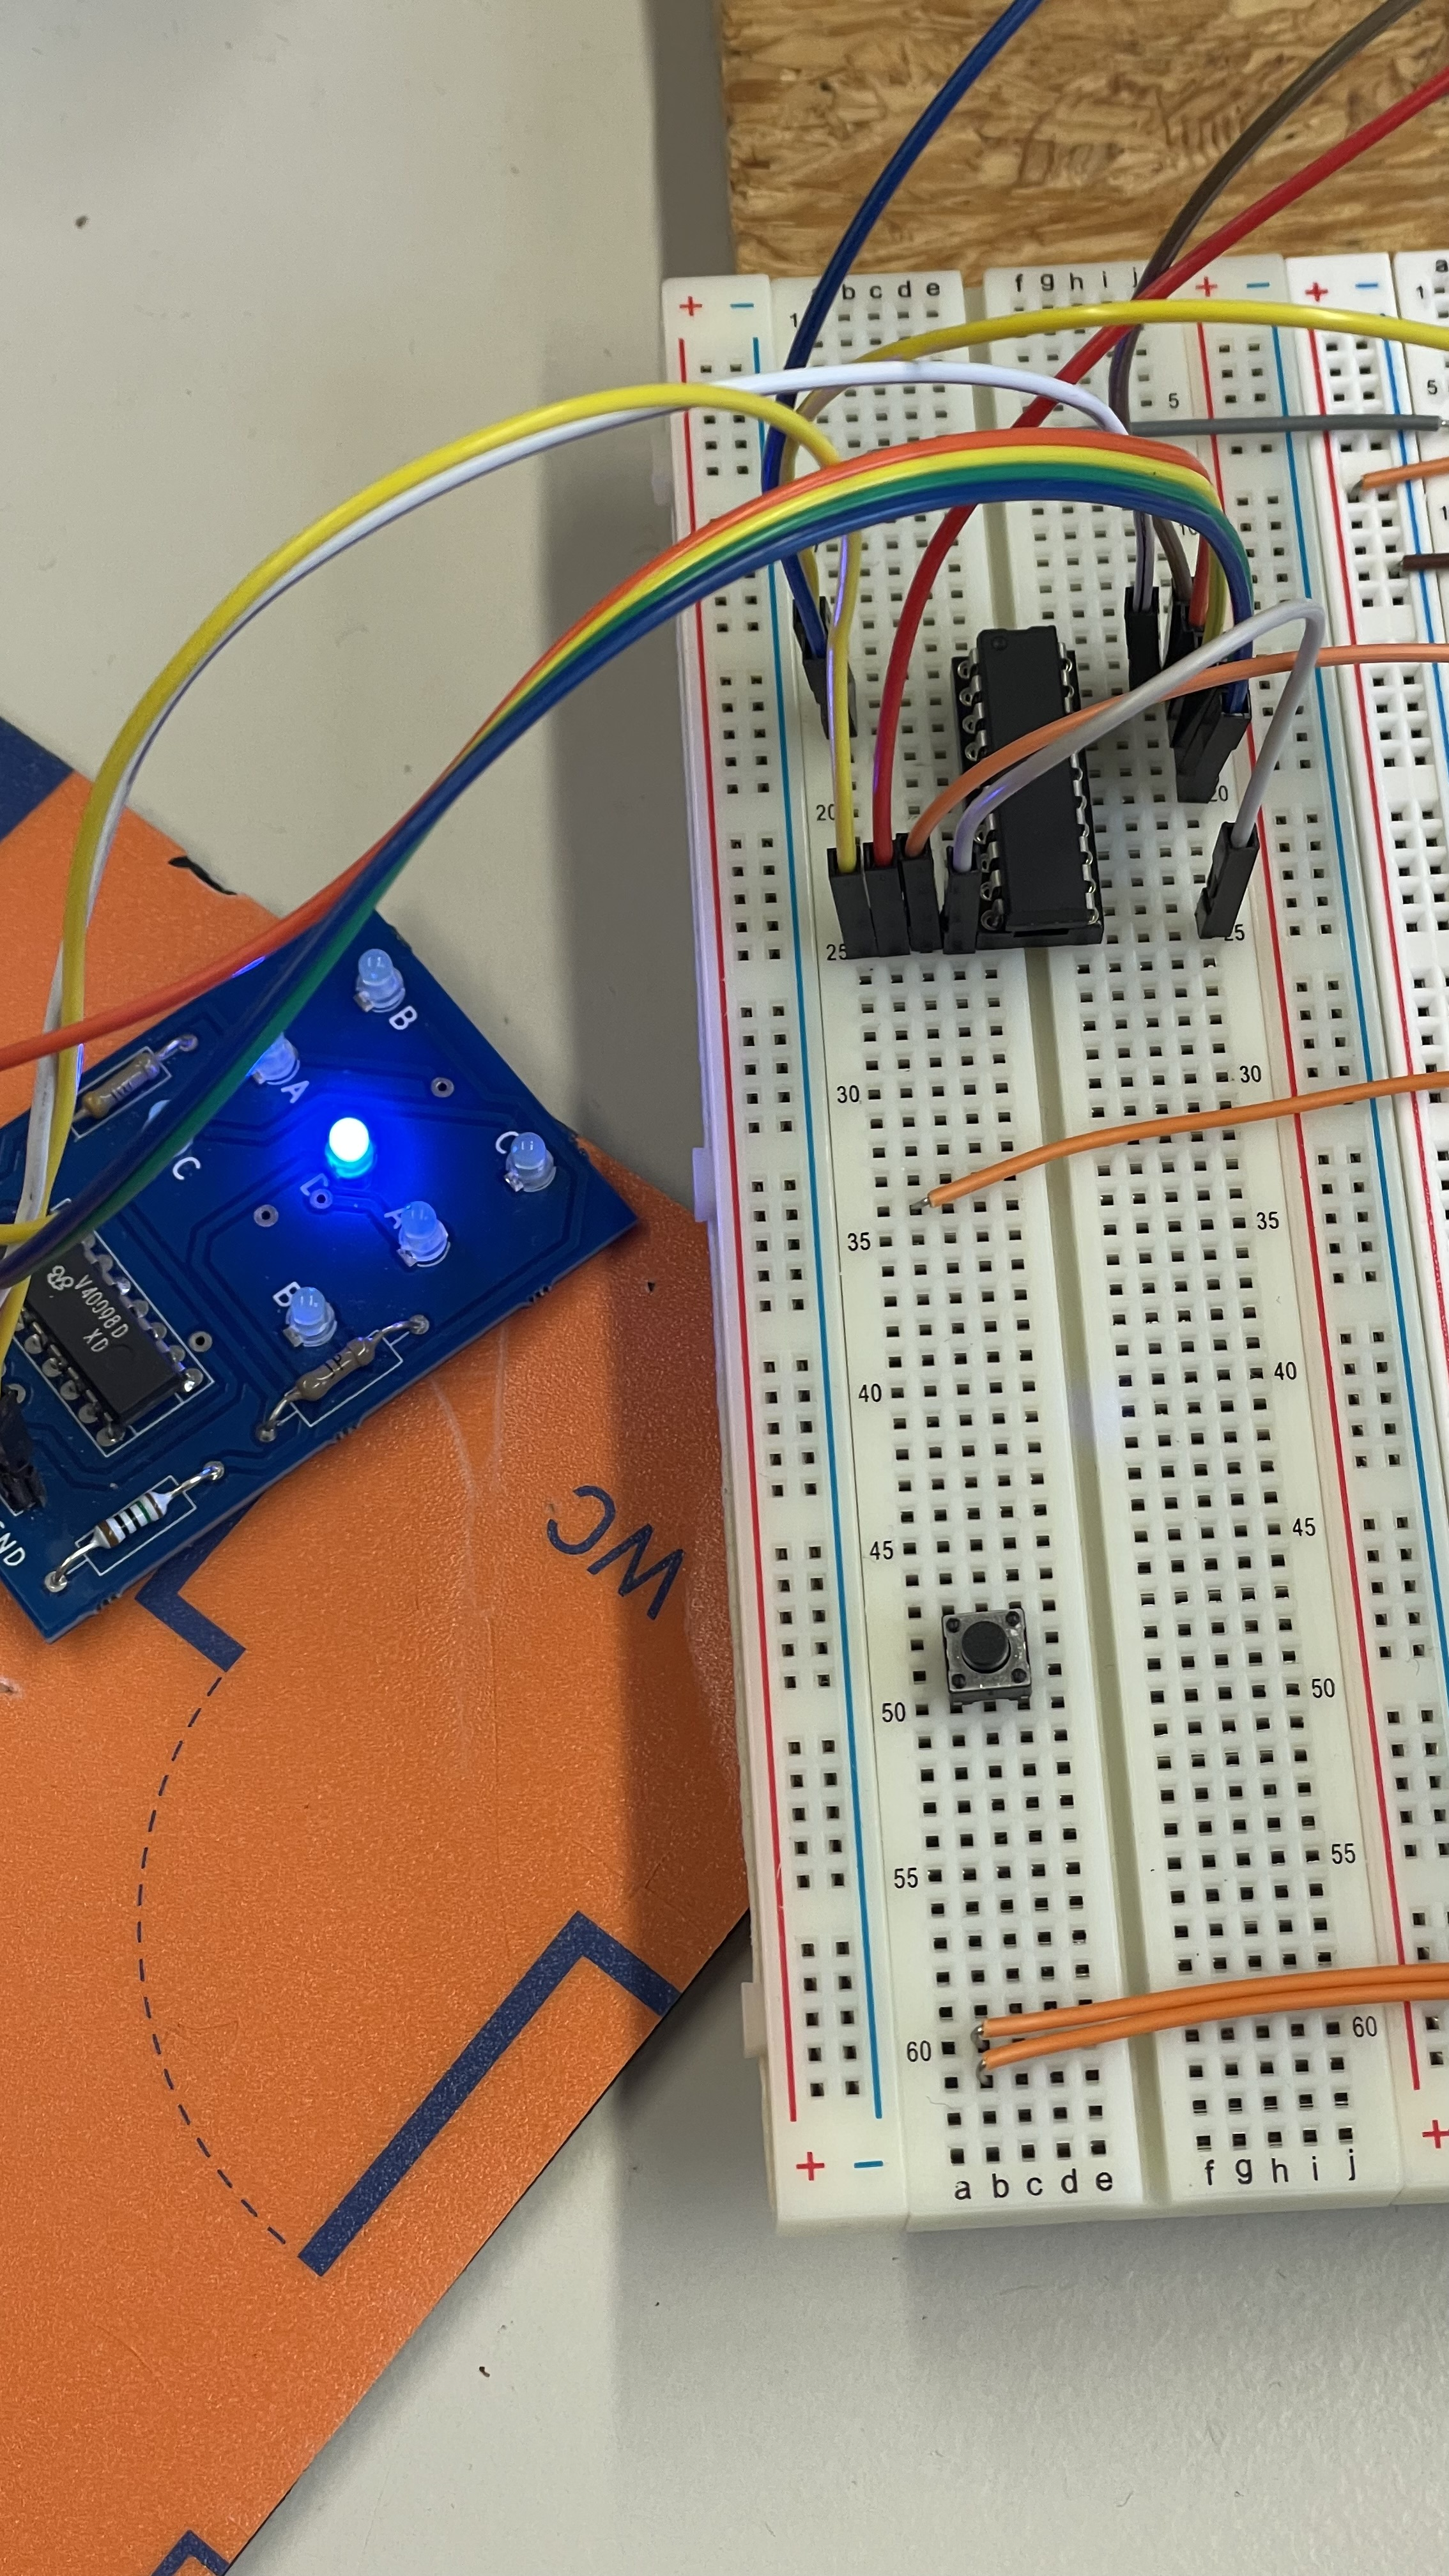
\includegraphics[width=0.8\textwidth]{dice_gal.jpeg}
     \label{fig:gal-setup}
\end{figure}